
You, OSDI PC member, probably have lots of gnitty gritty objections to why
this design isn't going to work, or isn't going to be useful. Well, we actually built this thing to prove
you wrong. Here are the engineering tricks we mustered to address the problems
you're thinking of.

Figure \ref{fig:system} depicts our architecture. We address the parts in turn:
\begin{figure*}[!t]
  \centering
  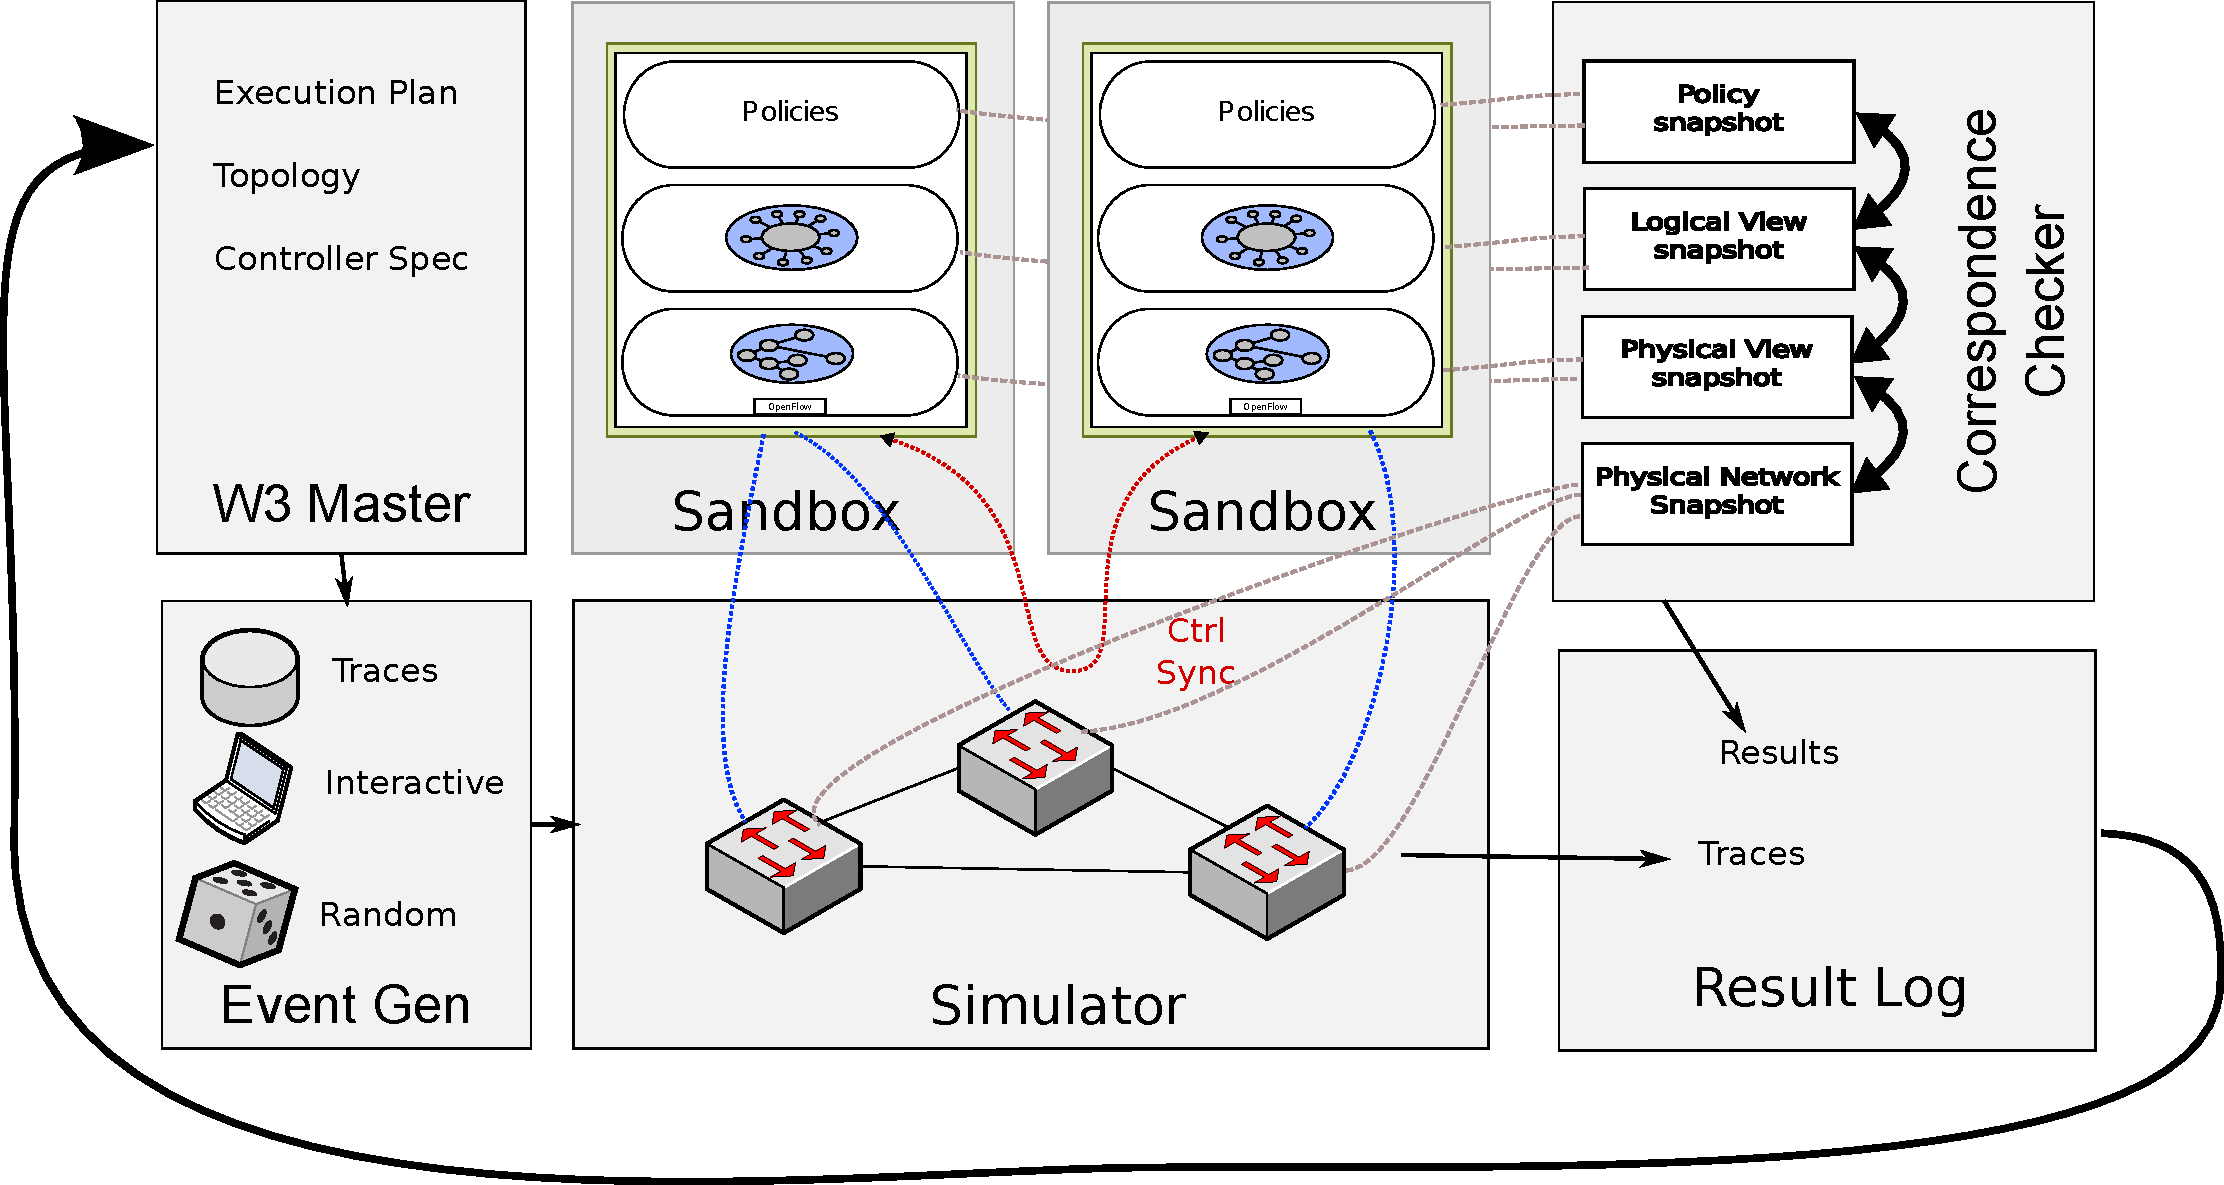
\includegraphics[width=0.8\textwidth]{../diagrams/architecture/architecture.pdf}
  \caption{System architecture}
  \label{fig:parallel_drops_master}
\end{figure*}

\noindent{\bf Event Generation} Event generation has two components.
We first generate system executions, which come from one of three sources:
\begin{enumerate}
\item traces taken from the real networks
\item synthetic traces. Real hosts running in VMs push traffic through our
network. The traces can also be fuzzed. 
\item Model checked traces, for example, found with NICE.
\end{enumerate}

We then select a subset of events to find pernicious policy-violations. Our
technique was described was described in \S\ref{sec:approach}.

\noindent{\bf Simulator} We model the following things: 
\begin{enumerate}
\item switch failures
\item link failures
\item packet re-orderings, drops, delays
\item naive packet forwarding
\item fully general control plane
\end{enumerate}

We can scale our simulation to datacenter-scale networks. We do that by using lightweight python objects. We don't have to worry
about dataplane forwarding! Only really have to model control plane and failures.

Each model switch keeps a TCP connection with the controller. This scales up
to X sockets.

Running the simulator in a single process gives us determinism. Determinism is
good, since we can rewind the execution, etc.

\noindent{\bf Controller Sandbox}

We can run whatever controller we want on top of the simulator!

The system execution has to be deterministic. Achieving determinism 
is a solved problem. There are a number of approaches, each with different
tradeoffs. Lightweight: use a software layer for determinism (random number
generators). No change in control software: binary instrumentation, jvm
tricks, full-blown VM replay.

By default, we run controllers in VMs. We can run these VMs on different
machines if we encounter memory or CPU bottlenecks.

If you want correspondence checking, you're going to have to give us your NOM.
Very small amount of code. We already have the protobuf serialization format
set up.

\noindent{\bf Correspondence Checking}

We modified the HSA code base. There is a ton of parallelization that can be
done to make it go fast!
